\begin{table}[H]
    {\renewcommand{\arraystretch}{1.3}%
    \setlength{\tabcolsep}{0.3em}%
    \begin{tabular}{bababab}
    \toprule
\rowcolor{white} \null &
\textbf{Synthetic$_{\mathbf{\mathcal{F}}}$} & \textbf{Synthetic$_{\mathbf{\mathcal{\beta}}}$} &
\textbf{Lehrpfad$_{\mathbf{\mathcal{F}}}$} & \textbf{Lehrpfad$_{\mathbf{\mathcal{\beta}}}$} &
\textbf{Office$_{\mathbf{\mathcal{F}}}$} & \textbf{Office$_{\mathbf{\mathcal{\beta}}}$}
\\
\midrule
\rowcolor{lightgray}
\textbf{Keypoint Count} &
    \num{217501} & \num{44309} &
    \num{2168195} & \num{2198582} &
    \num{171000} & \num{171000}
    \\
\textbf{Correspondences} &
    \num{96374} & \num{26466} &
    \num{298093} & \num{222505} &
    \num{43057} & \num{36331}
    \\
\rowcolor{lightgray}
\textbf{True Positives} &
    \num{76614} & \num{22289} &
    \num{110358} & \num{35467} &
    \num{24026} & \num{15454}
    \\
\textbf{False Positives} &
    \num{59017} & \num{8883} &
    \num{648653} & \num{650897} &
    \num{48823} & \num{48756}
    \\
    \bottomrule
    \end{tabular}
    }
    \caption{Performance indicators for the default configuration of the SIFT algorithm on the different datasets.}
\end{table}

\begin{figure}[H]
\begin{subfigure}[t]{0.45\linewidth}
    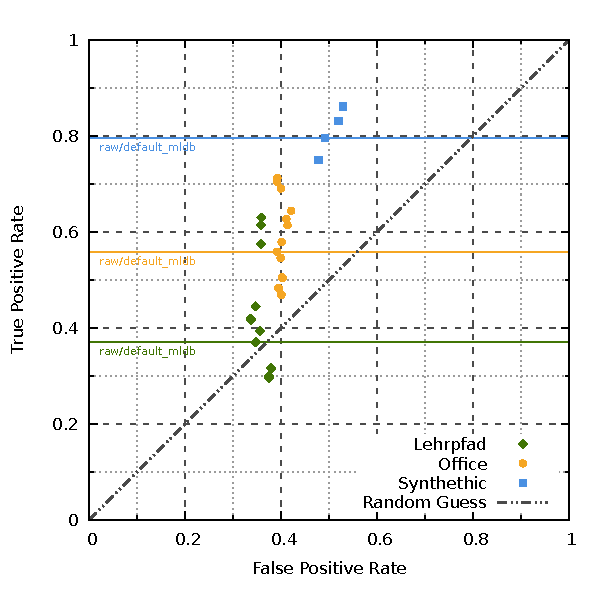
\includegraphics[width=\linewidth]{chapter06/results/AKAZE/flexion/roc.pdf}%
    \caption{Flexion Image ROC}
\end{subfigure}\quad
\begin{subfigure}[t]{0.45\linewidth}
    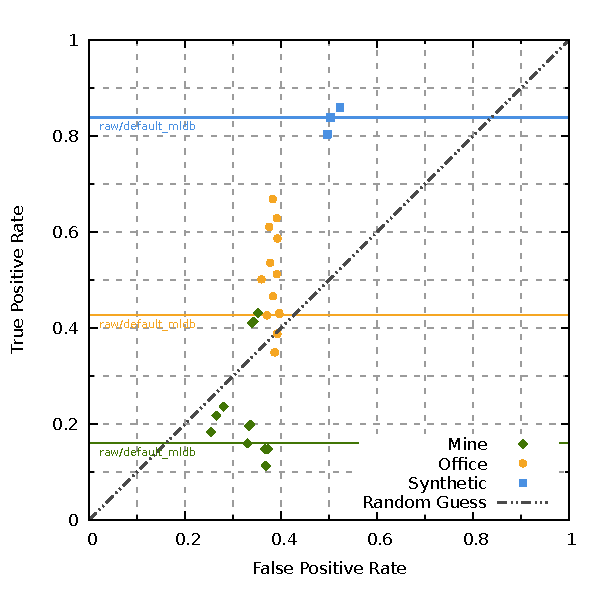
\includegraphics[width=\linewidth]{chapter06/results/AKAZE/bearing/roc.pdf}
    \caption{Bearing-Angle Image ROC}
\end{subfigure}
    \caption{AKAZE}
\end{figure}

\begin{figure}[H]
\begin{subfigure}[t]{0.45\linewidth}
    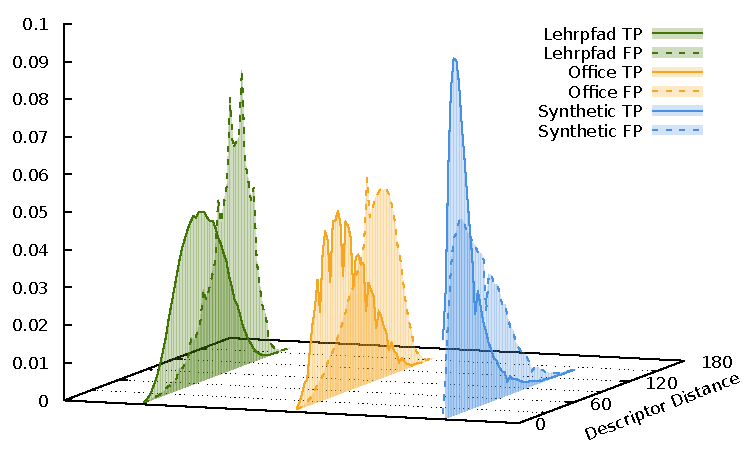
\includegraphics[width=\linewidth]{chapter06/results/AKAZE/flexion/descriptor_distances.pdf}%
    \caption{\gls{flexion-image} Descriptor Distances}
\end{subfigure}\quad
\begin{subfigure}[t]{0.45\linewidth}
    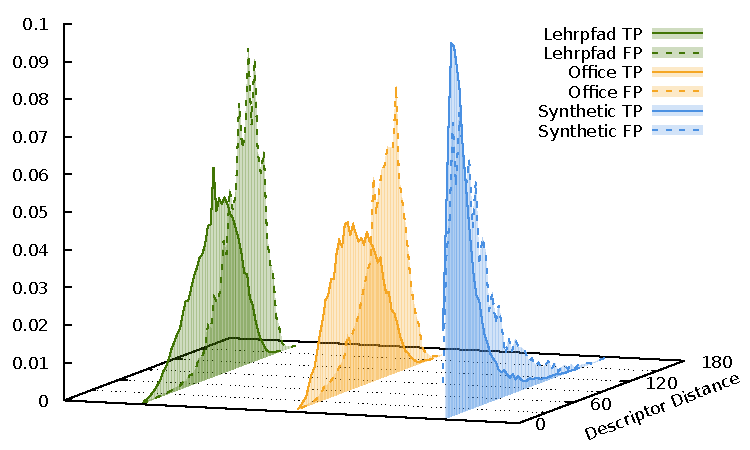
\includegraphics[width=\linewidth]{chapter06/results/AKAZE/bearing/descriptor_distances.pdf}%
    \caption{\gls{bearing-angle-image} Descriptors Distances}
\end{subfigure}
\end{figure}
